\section{Results}
\label{sec:results}

%\emph{Benchmarks (test results) and possibly competition results.  Include explanations and analyses of your results. As mentioned under “Benchmarks and comparisons” below, it is usually a clear strength if you have some results to com- pare, e.g. two different versions of your client with different methods/features/parameters.  You could also compare the behaviour of your client on different individual levels that illustrate a certain point, e.g. similar levels resulting in large differences in the client’s behaviour.}

To showcase how our goal prioritization works, and how we have improved upon it throughout the project, we have run the level SAOptimal with different levels of complexity in the prioritization.
Our client can run a level with a simple and a complex goal prioritization. 

The simple goal prioritization will use the first step of the goal prioritization technique described in \cref{methods:goal_ordering}. 
This will prioritize the goals placed in dead-ends or corners, higher than goals with adjacent free cells or other goal cells.

The problem with this technique can be seen in \cref{fig:SAOptimal}. 
The goals r and s, will have the same priority because they both have 3 goal cells and a wall adjacent to them. 
Therefore, the AI might pick r before s, causing s to be blocked off. 
The agent will then have to move the R box again in order to place the S box in the s goal causing an increase in actions taken.

% Example of cells 
\begin{figure}[h!]
  \centering
  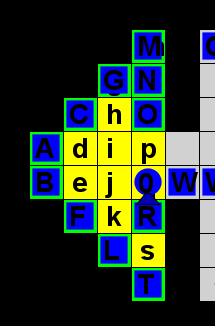
\includegraphics[width=.5\columnwidth]{graphics/simple_priority_block.png}
  \caption{\label{fig:SAOptimal}Simple prioritization blocking of s.}
\end{figure}

This is fixed in the complex goal prioritization, where the AI is told to choose the exact order in which the goals are prioritized, placing goals that will be blocked off higher than then goals that will block them.  
The improvements from the simple to the complex goal prioritization is illustrated in \cref{tab:SAOptimal_results}, where the results of the two runs are shown.

\begin{table}[h!]
\centering
\caption{SAOptimal Results}
\label{SAOptimal_results}
\begin{tabular}{| l | l |}
\hline
                                   & Actions\\ \hline
Simple prioritization    & 761      \\ \hline
Complex prioritization & 730     \\ \hline
\end{tabular}
\end{table}

